\RequirePackage{luatex85}
\documentclass[border=1mm]{standalone}
\usepackage{myFig}
\begin{document}
	\begin{tikzpicture}
		\def\largearrow#1#2{

			\coordinate (arrow#1-left)  at ($(#2) - (0.75, 0)$);
			\coordinate (arrow#1-right) at ($(#2) + (0.75, 0)$);

			\draw (arrow#1-left)  -- ++( 0.25,  0.25) coordinate (al-above);
			\draw (arrow#1-left)  -- ++( 0.25, -0.25) coordinate (al-below);
			\draw (arrow#1-right) -- ++(-0.25,  0.25) coordinate (ar-above);
			\draw (arrow#1-right) -- ++(-0.25, -0.25) coordinate (ar-below);

			\draw ($(arrow#1-left)!0.5!(al-above)$) -- ($(arrow#1-right)!0.5!(ar-above)$);
			\draw ($(arrow#1-left)!0.5!(al-below)$) -- ($(arrow#1-right)!0.5!(ar-below)$);
		}
		\node[align=center, draw, anchor=south] (CPU) at (0, 7.5*1.4) {CPU\\(計算,制御)};
		\draw ($(0, 0)-(0.5, 0)$) rectangle ($(CPU.south)+(0.5, 0)$);
		\node[align=center, draw, anchor=west] (memory) at (2, 7*1.4) {主記憶装置/メモリ\\(プログラム、データ)};
		\node[align=center, draw, anchor=west] (interface1) at (2, 6*1.4) {インタフェース回路};
		\node[align=center, draw, anchor=west] (interface2) at (2, 5*1.4) {インタフェース回路};
		\node[align=center, draw, anchor=west] (interface3) at (2, 4*1.4) {インタフェース回路};
		\node[align=center, draw, anchor=west] (interface4) at (2, 3*1.4) {インタフェース回路};
		\node[align=center, draw, anchor=west] (interface5) at (2, 2*1.4) {インタフェース回路};
		\node[align=center, draw, anchor=west] (interface6) at (2, 1*1.4) {インタフェース回路};
		
		\largearrow{7}{[xshift=-0.75cm]memory.west};
		\largearrow{1-1}{[xshift=-0.75cm]interface1.west};
		\largearrow{2-1}{[xshift=-0.75cm]interface2.west};
		\largearrow{3-1}{[xshift=-0.75cm]interface3.west};
		\largearrow{4-1}{[xshift=-0.75cm]interface4.west};
		\largearrow{5-1}{[xshift=-0.75cm]interface5.west};
		\largearrow{6-1}{[xshift=-0.75cm]interface6.west};
		
		\largearrow{1-2}{[xshift=0.75cm]interface1.east};
		\largearrow{2-2}{[xshift=0.75cm]interface2.east};
		\largearrow{3-2}{[xshift=0.75cm]interface3.east};
		\largearrow{4-2}{[xshift=0.75cm]interface4.east};
		\largearrow{5-2}{[xshift=0.75cm]interface5.east};
		\largearrow{6-2}{[xshift=0.75cm]interface6.east};

		\node[anchor=west, inner sep=0pt] (timer) at (arrow1-2-right) {
			\begin{tikzpicture}
				\draw (0, 0) circle[radius=0.6cm];
				\draw[-latex] (0, 0) -- (0, 0.6);
				\draw[-latex] (0, 0) -- (0.6, 0);
			\end{tikzpicture}
		};
		
		\node[anchor=west, inner sep=0pt] (harddisk) at (arrow2-2-right) {
			\begin{tikzpicture}
				\node[anchor=south, align=center] at (0, 0) {ハード\\ディスク};
				\draw (-0.75, 0) -- ++(0, 1);
				\draw ( 0.75, 0) -- ++(0, 1);
				\draw (0, 1) circle [x radius=0.75cm, y radius=0.2cm];
				\draw (-0.75, 0) arc [x radius=0.75cm, y radius=0.2cm, start angle=180, end angle=360];
			\end{tikzpicture}
		};
		
		\node[anchor=west, inner sep=0pt] (cd-rom) at (arrow3-2-right) {
			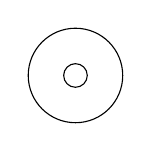
\begin{tikzpicture}
				\draw (0, 0) circle[radius=0.6cm];
				\draw (0, 0) circle[radius=0.15cm];
			\end{tikzpicture}
		};
		
		\node[anchor=west, inner sep=0pt] (keyboard) at (arrow4-2-right) {
			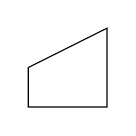
\begin{tikzpicture}
				\draw (0, 0) -- (0, 0.5) -- (1, 1) -- (1, 0) -- cycle;
			\end{tikzpicture}
		};

		\node[anchor=west, inner sep=0pt] (display) at (arrow5-2-right) {
			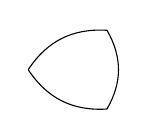
\begin{tikzpicture}
				\draw (0, 0) to[bend left] (1, 0.5) to[bend left] (1, -0.5) to[bend left] (0, 0);
			\end{tikzpicture}
		};

		\node[anchor=west, inner sep=0pt] (network) at (arrow6-2-right) {
			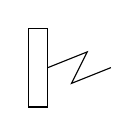
\begin{tikzpicture}
				\draw (0, 0) rectangle (0.25, 1);
				\draw (0.25, 0.5) -- ++(0.5, 0.2) -- ++(-0.2, -0.4) -- ++(0.5, 0.2);
			\end{tikzpicture}
		};

		\node[anchor=west, align=center] at (timer.east) {時計/タイマ};
		\node[anchor=west, align=center] at (cd-rom.east) {CD-ROM};
		\node[anchor=west, align=center] at (keyboard.east) {キーボード};
		\node[anchor=west, align=center] at (display.east) {ディスプレイ};
		\node[anchor=west, align=center] at (network.east) {ネットワーク};
		
		\coordinate (io-inter) at ($(interface6.south) + (0, -1)$);
		\coordinate (io-equip) at ($(interface6.south) + (4.5, -1)$);

		\draw[dashed] ($(io-inter) - (2, 0)$) rectangle ($(io-inter) + (2, 6.5 * 1.4)$);
		\draw[dashed] ($(io-equip) - (2, 0)$) rectangle ($(io-equip) + (2, 6.5 * 1.4)$);
		\node[anchor=north] at (io-inter.south) {入出力インターフェース};
		\node[anchor=north] at (io-equip.south) {入出力装置};
		
		\draw[dotted, line width=2pt] ([yshift=2mm]io-inter) -- ++(0, 0.5);
		
		\node[rotate=-90] at (0, 6) {バス};
		
		

	\end{tikzpicture}
\end{document}
